% \documentclass[12pt,a4paper]{article}
% \usepackage[italian]{babel}
% \usepackage[utf8]{inputenc}
% \usepackage[]{graphicx}
% \usepackage{newlfont}
% \usepackage{sidecap}
% \usepackage{enumerate}
% \usepackage{natbib}
% \usepackage{amssymb}
% \usepackage{tikz}
% \usepackage{hyperref}
% \usepackage{xcolor}
% \usepackage{colortbl}
% \usepackage{midpage}

\newcommand{\tabitem}{~~\llap{\textbullet}~~}

% \begin{document}
\chapter{Localization}\label{sec3}

\section{Location and Location-Based Services}\label{subsec3.1}

Le tecnologie di localizzazione sono una combinazione di metodi e
tecniche che permettono di individuare la posizione di un oggetto o di una
persona nel mondo reale. I servizi location-based sono servizi specifici che si
basano sulla posizione. Un'applicazione molto comune che utilizza questo genere
di servizi è Google Maps.
Affinché funzionino correttamente e in modo efficiente, queste tecniche
di localizzazione richiedono:
\begin{itemize}
   \item Accuratezza: ovvero la posizione deve essere precisa con
un minimo errore.
    \item Costo: stabilire cosa conviene utilizzare tra GPS o una
localizzazione interna. Ci sono casi in cui è conveniente inserire più nodi
piuttosto che metterne meno, ma più costosi.
    \item Distribuzione
    \item Ubiquità
    \item Requisiti specifici di un'applicazione
\end{itemize}
Non è sempre possibile soddisfarli tutti contemporaneamente, infatti
molti di questi sono in conflitto tra loro.

Bisogna tener conto di tutte queste considerazioni nello sviluppo di
metodologie di localizzazione, soprattutto quando si entra nell'ambito di
sistemi cyber-fisici.
Questi sistemi comprendono due blocchi principali:
\begin{itemize}
    \item Dei nodi in stati differenti:
    \begin{itemize}
        \item Unknown: localizzazione non conosciuta
        \item Settled: la posizione dei nodi è nota e essi
            possono aiutare a scoprire la posizione di altri nodi
        \item Beacon: nodi landmark, possono essere statici
            $\rightarrow$ il satellite è un beacon node; esso manda in broadcast le
            informazioni che possono essere usate dal GPS Receiver per determinare la
            posizione dell'oggetto
    \end{itemize}
    \item Un algoritmo di localizzazione per determinare la
        posizione del nodo unknown.
\end{itemize}

\section{Il GPS è l'unica scelta possibile?}\label{subsubsec3.1.1}
Il GPS non sempre è la soluzione più conveniente; per esempio
esso funziona solo outdoor e consuma molta energia.
L'alto consumo energetico è dovuto al fatto che la comunicazione è molto lenta
e questo significa che l'antenna per al trasmissione delle informazioni resta
attiva più a lungo con un conseguente alto consumo di energia.
Questo problema va poi moltiplicato per 3 poiché bisogna comunicare con almeno
3 anchor nodes.
Sono quindi state proposte altre tecniche per stabilire la
posizione dei nodi sconosciuti. Esse sfruttano:
\begin{itemize}
    \item Sensing Capabilities: sfruttano la propagazione di onde radio, la
    forza di ricezione del segnale (RSSI), il tempo di arrivo (ToA) ecc..
    \item Comunicazione Wireless
\end{itemize}

\section{Tecnologie Disponibili e Possibili Scenari di Utilizzo}\label{subsec3.2}

Le tecnologie di localizzazione sono molto numerose, tra le più famose abbiamo:
\begin{itemize}
    \item GPS Galileo: alternativa europea che è molto più precisa
        rispetto al classico GPS perché sfrutta il clock. Esso però presenta alcuni
        problemi sistematici che dovrebbero essere risolti tra il 2020 e il 2021.
    \item Wi-Fi Beacons: si utilizzano molti database per sapere la
        posizioni basandosi sulle informazioni degli access-point. Essa offre una misura
        più accurata di quella satellitare, a patto che si abbia un access-point
        disponibile.
    \item Tecnologia acustiche che sfruttano altre proprietà
        fisiche.
\end{itemize}

Esistono molte applicazioni possibili per la localizzazione, come ad
esempio localizzare i pazienti all'interno di un ospedale, localizzazione di
opere d'arte nei musei o delle componenti in una catena di montaggio di una
azienda.

\section{Localization Taxonomy}\label{subsec3.3}
\begin{figure}
    \centering
    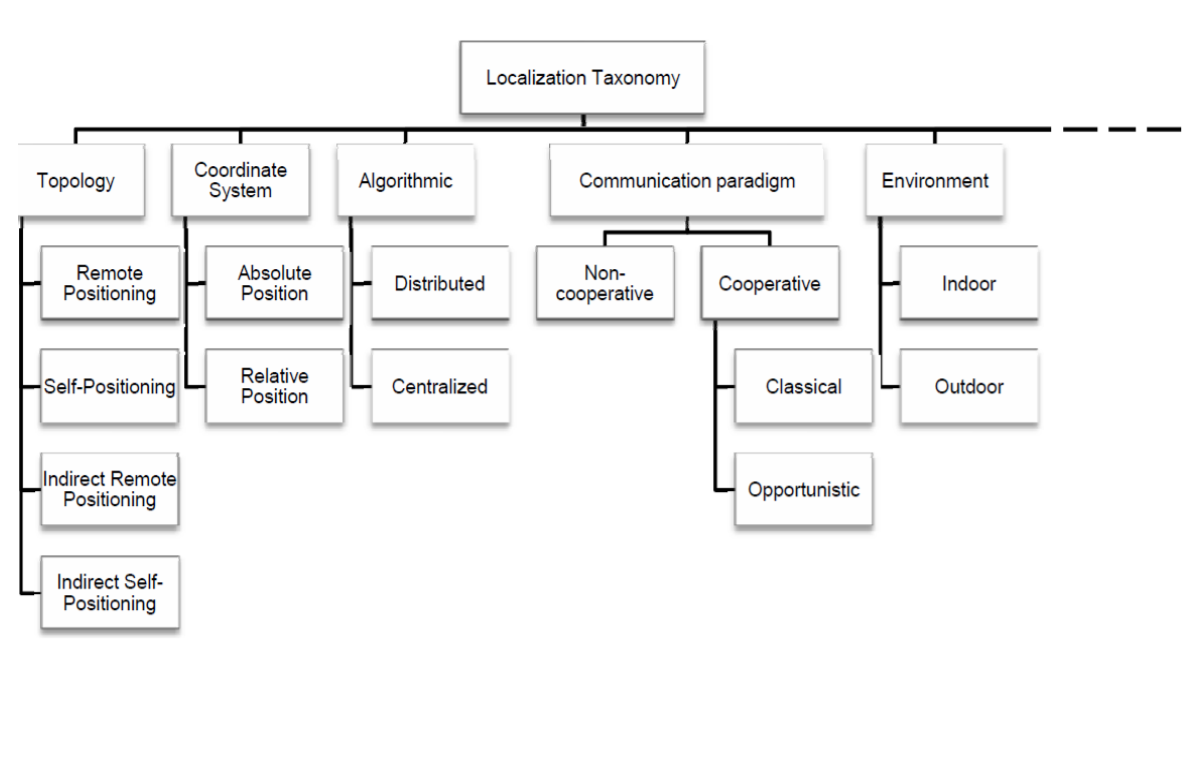
\includegraphics[scale=0.5]{fig1-lec3pt1.png}
    \caption{Tassonomia}
    \label{fig:fig1-lec3pt1}
\end{figure}

La tassonomia come si vede in Fig.~\ref{fig:fig1-lec3pt1} è molto vasta:

\begin{itemize}
    \item Topologia: dove e come viene calcolata la posizione di un
    nodo. Possiamo avere 4 tipi di topologia:
    \begin{itemize}
        \item Remote Positioning: un nodo sconosciuto
        manda messaggi broadcast che vengono ricevuti da un anchor node; l'informazione
        viene poi mandata alla base station che la rimanda al nodo sconosciuto. Remote
        positioning può essere usato per il tracking degli animali selvaggi.
        \item Self-Positioning (ad esempio il GPS): il
        nodo si calcola la propria posizione sulla base delle informazioni ricevute dal
        nodo anchor.
        \item Indirect Remote Positioning: simile al
        self-positioning. È disponibile un ulteriore canale di comunicazione tra il nodo
        e la base station.
        \item Indirect Self-Positioning: simile al
        remote positioning. La base station calcola la posizione e la inoltra al nodo
        interessato.
    \end{itemize}
    \item Coordinate System: la posizione viene rappresentata in un
    sistema di coordinate. Può essere assoluta, ovvero espressa attraverso
    coordinate uniche che fanno riferimento ad un nodo anchor (e.g. GPS), oppure
    relativa con sistema di riferimento relativo ad altri nodi che non sono anchor.
    \item Algoritmi: si dividono in:
    \begin{itemize}
        \item Centralizzati: c'è un dispositivo centrale (ad
        esempio la base station) che si occupa del calcolo della posizione dei nodi
        sconosciuti. Ciò comporta che bisogna basarsi su informazioni globali per il
        calcolo della posizione, miglior accuratezza a discapito dell'alto costo
        computazionale e consumo energetico, problemi di scalabilità ed efficienza
        computazionale.
        \item Distribuiti: i nodi calcolano la posizione
        autonomamente grazie alle informazioni raccolte dai nodi anchor. Con questo
        metodo si riduce la complessità e si migliora l'efficienza energetica.
    \end{itemize}

    \begin{figure}
            \centering
            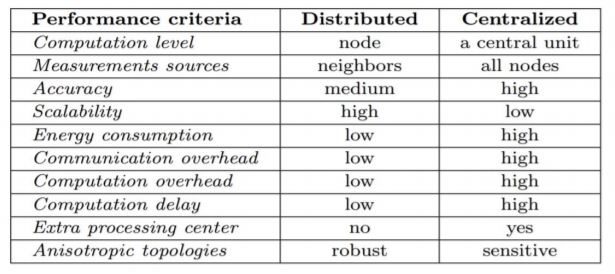
\includegraphics[scale=0.6]{fig2-lec3pt1.png}
            \caption{Differenza tra centralizzato e decentralizzato}
            \label{fig:fig2-lec3pt1.png}
    \end{figure}
    \item Environment: outdoor o indoor
    \item Paradigma di Comunicazione: modo in cui i nodi comunicano
    tra di loro:
    \begin{itemize}
        \item Non-Cooperative: la comunicazione è limitata tra
        nodi sconosciuti e nodi anchor. È necessario garantire un numero minimo di nodi
        anchor e poi si può decidere se disporre i nodi anchor in grande densità oppure
        sfruttare degli anchor a trasmissione a lungo raggio.
        \item Cooperative: non ci sono restrizioni e non c'\`e
        bisogno di alta densità di nodi anchor, ma è richiesta un'alta
        intensità di processamento delle operazioni in modo da filtrare le
        misure disturbate.
        \item Opportunistic: sfrutta un contatto non programmato
        per inferire la posizione di un nodo. Un esempio è l'RFID.
    \end{itemize}
\end{itemize}

\section{Localization Categories}\label{subsec3.4}

Abbiamo diverse categorie come si può notare in
Fig.~\ref{fig:fig3-lec3pt1}
\begin{figure}
        \centering
        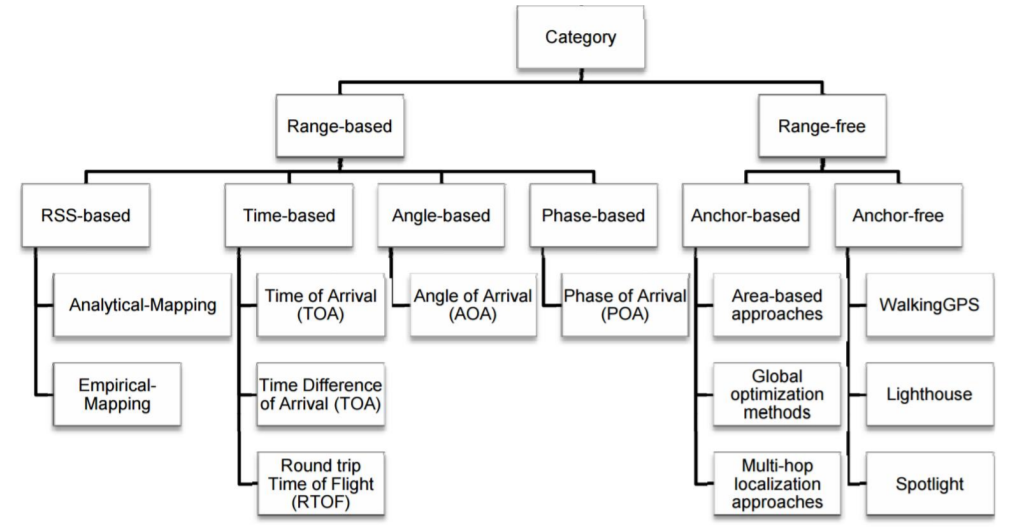
\includegraphics[scale=0.6]{fig3-lec3pt1.png}
        \caption{Categorie}
        \label{fig:fig3-lec3pt1}
\end{figure}
Abbiamo due macro categorie che sono Range-Based e Range-Free.
Le tecniche Range-Based effettuano misurazioni sulla distanza per
calcolare la posizione dei nodi sconosciuti sfruttando ad esempio la potenza del
segnale e il tempo: in questo modo si riesce a sapere la distanza dei nodi che
entrano a far parte della comunicazione e combinando 3 nodi si può individuare
la posizione. Le tecniche Range-Free invece fanno riferimento alla posizione
relativa tra due nodi (opportunistic).

\subsection{Range-Based}\label{subsubsec3.4.1}
\begin{itemize}
    \item \textbf{RSS-Based techinque}: tecnica che prevede di creare un
    mapping tra la distanza e la potenza di segnale ricevuta (RSS = Received Signal
    Strength). Generalmente si calcola l'RSS in modo semplificato conoscendo
    l'RSS a una distanza di riferimento combinata con un parametro che
    dipende dall'ambiente. C'è però un problema dovuto al fatto che si
    assume che il segnale abbia un'andamento a campana, ma gli esperimenti
    hanno dimostrato che invece ha un andamento molto variabile.
    \begin{itemize}
        \item Analytical-Mapping: la distanza RSS viene mappata da
        un'equazione matematica.
        \item Empirical Mapping: la distanza RSS viene mappata
        attraverso analisi statistica dei dati. Questo tipo di tecnica è molto usata in
        robotica e nel campo dell'automazione. Inizialmente si effettua una
        RSS-Gathering e si costruisce la mappa. Un'entità autonoma misura l'RSS e
        interroga la mappa; a questo punto viene inferita la posizione effettiva.
    \end{itemize}

    \begin{centering}
        \begin{tabularx}{\textwidth}{|l|X|X|}
            \hline
            Tecniche & Pro & Contro \\
            \hline
            ~Analytical-Mapping & \tabitem Facile da implementare & \tabitem I parametri dipendono dall'ambiente \\
            & \tabitem Utile per il design dei simulatori & \tabitem Scarsa precisione \\
            \hline
            ~Empirical-Mapping & \tabitem Può raggiungere un alto livello di accuratezza & \tabitem È necessario un ulteriore profiling dell'ambiente \\
            & & \tabitem Alto overhead nella computazione offline \\
            & & \tabitem Scarsa scalabilità \\
            & & \tabitem Inaffidabile in ambienti dinamici \\
            \hline
        \end{tabularx}
    \end{centering}


    \item \textbf{Time-Based techinque}: la stima della posizione viene effettuata tenendo conto
    del tempo di propagazione del segnale radio.
    \begin{itemize}
        \item Time of Arrival (ToA): si conta il tempo di propagazione tra due
        nodi sincronizzati (sender e receiver devono essere sincronizzati).

		\textit{Funzionamento}: il sender (nodo ancora) invia ad intervalli regolari un beacon; il nodo receiver (unknown) essendo sincronizzato con l'ancora, sa quando è stato inviato il pacchetto e calcola la distanza in base al ritardo con il quale l'ha ricevuto.

        Questi metodi sono poco utilizzati perché richiedono hardware costosi e grosse capacità
        di computazione. Un esempio di applicazione è il sistema GPS a larga distanza
        con un alta risoluzione di clock.

        \item Round-trip Time of Flight (RFOT): strategia alternativa che evita la
        sincronizzazione dei nodi. \`E possibile determinare la posizione solo conoscendo
        la velocità del protocollo usato che può essere noto, calcolato statisticamente
        o comunicato dal nodo.

        \textit{Funzionamento}: il nodo unknown manda un beacon, i nodi ancora che lo ricevono glielo re-inviano; la distanza viene calcolata dal nodo unknown tenendo conto del tempo impiegato dai vari pacchetti per tornare.

        \item Time Difference of Arrival (TDoA): il nodo che deve inferire la posizione riceve dai nodi ancora due segnali a frequenze diverse, tipicamente uno radio e uno ultrasuono, e calcola la distanza in base alla differenza d'arrivo dei due segnali, prendendo come riferimento il più veloce (\textbf{Single Receiver}).
        Così facendo non serve la sincronizzazione dei nodi, il consumo di
energia è ridotto ma sono necessarie più antenne.

        In alternativa è possibile utilizzare due ricevitori posti ad una distanza nota ed approssimare la distanza dalla sorgente utilizzando la differenza nel tempo di ricezione del segnale da parte dei due ricevitori (\textbf{Multiple Receiver}).
        In questo caso viene utilizzato un singolo segnale.
    \end{itemize}
    \item \textbf{Angle of Arrival}: viene utilizzato l'angolo di arrivo del segnale per capire in che direzione si trova il nodo sconosciuto rispetto all'ancora dalla quale ha ricevuto il segnale.

    Se è disponibile l'informazione riguardo l'orientamento delle varie ancore bastano solo due nodi ancora per inferire la posizione, altrimenti ne sono necessari tre.

    Per determinare l’angolo di arrivo di un segnale si può utilizzare un'antenna rotante (hardware costoso) oppure un array di antenne poste a distanza fissa tra loro in modo da determinare l'angolo in base a come queste ricevono il segnale.

    Una volta determinati i vari angoli di arrivo del segnale, si risolve un sistema di equazioni lineari per determinare la posizione relativa dell'oggetto.
\end{itemize}

\begin{figure}
        \centering
        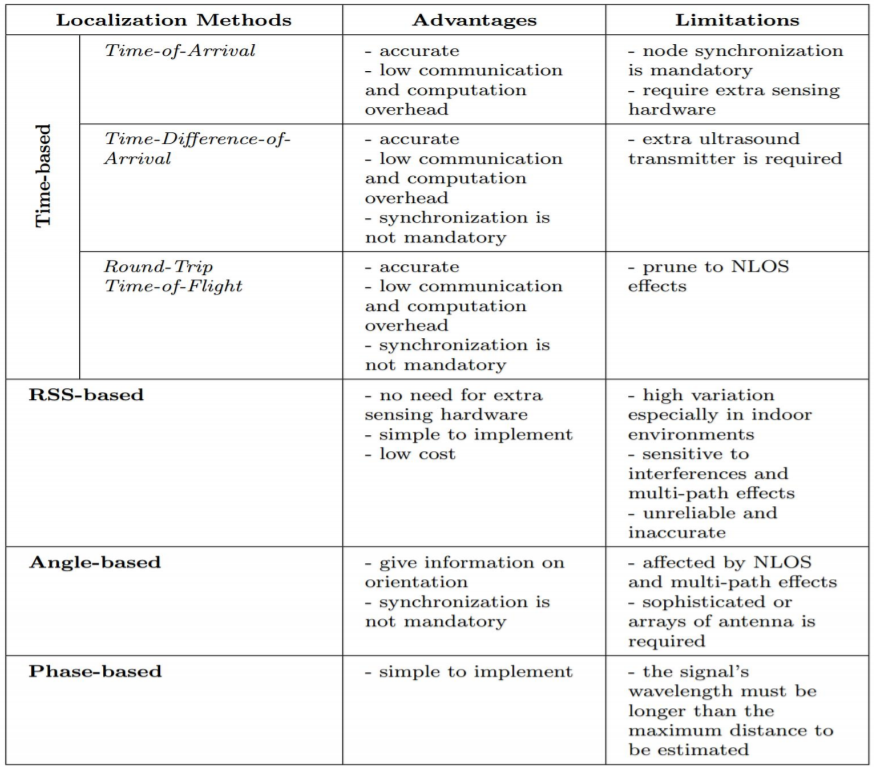
\includegraphics[scale=0.55]{fig4-lec3pt1.png}
        \caption{Range-Based Comparison}
        \label{fig:fig4-lec3pt1}
\end{figure}


\subsection{Range-Free}\label{subsubsec3.4.2}
\begin{itemize}
    \item \textbf{Anchor-Based}: vengono predisposti dei nodi ancora in posizioni note che inviano in broadcast la loro posizione. I nodi unknown calcolano la loro posizione utilizzando i messaggi ricevuti dalle ancore alla quali riescono a connettersi\footnote{\url{http://journals.sagepub.com/doi/full/10.1155/2013/304628} §4 e §5}.

    Abbiamo diversi approcci:
    \begin{itemize}
        \item Area-Based: in cui la posizione viene calcolata
        come il baricentro dell'area del poligono che ha nei vertici i nodi.
        Un'alternativa è suddividere tale area in tanti triangoli e la posizione e
        l'intersezione di tutti i triangoli; il punto è il centro di massa
        dell'intersezione trovata.
        \item Multihop Localization: non è sempre possibile che
        il nodo target sia nel range di comunicazione con il numero minimo di nodi
        anchor richiesti per determinare la posizione.

        In questi casi si può utilizzare l'approccio \textbf{DV-HOP}:
        i nodi anchor mandano in broadcast un messaggio contenente la loro posizione ed un hop count $(X_i, Y_i, h_i)$; quando un nodo anchor riceve un messaggio da un'altro nodo anchor, lo rimanda in broadcast, aumentando di uno l'hop count.
        Così facendo quando un nodo unknown si connette ad un nodo anchor riceve anche i messaggi broadcast inviati dalle ancore fuori range. Con queste informazioni il nodo unknown riesce a stimare la sua distanza dai nodi anchor fuori range (\textit{1-hop distance estimation})\footnote{Da notare che la stima \textit{1-hop} può essere fatta direttamente dal nodo unknown (come descritto) oppure può essere fatta dai nodi ancora.}.

        DV-HOP funziona bene in topologia di rete isotropiche,
        ma è difficile da mettere in pratica per via degli ostacoli nell'ambiente,
        irregolarità del segnale radio e non uniformità della densità dei nodi.
    \end{itemize}
    \item \textbf{Anchor-Free}: metodo guidato dagli eventi che sfrutta
    proprietà spaziali e temporali degli eventi per inferire la posizione.
    Funziona sotto l'assunzione che alcuni eventi possono essere generati in un preciso istante e in una precisa posizione.
    Alcuni esempi di questo approccio sono \textbf{WalkingGPS} (un nodo mobile dotato di GPS fa il broadcast della sua posizione) o \textbf{Lighthouse}
\end{itemize}


\section{Tecniche di Geolocalizzazione}\label{subsec3.5}
Queste tecniche consento di trovare la posizione di un nodo basandosi
sull'informazione riguardante la misura della distanza o dell'angolo.
\begin{figure}
    \centering
    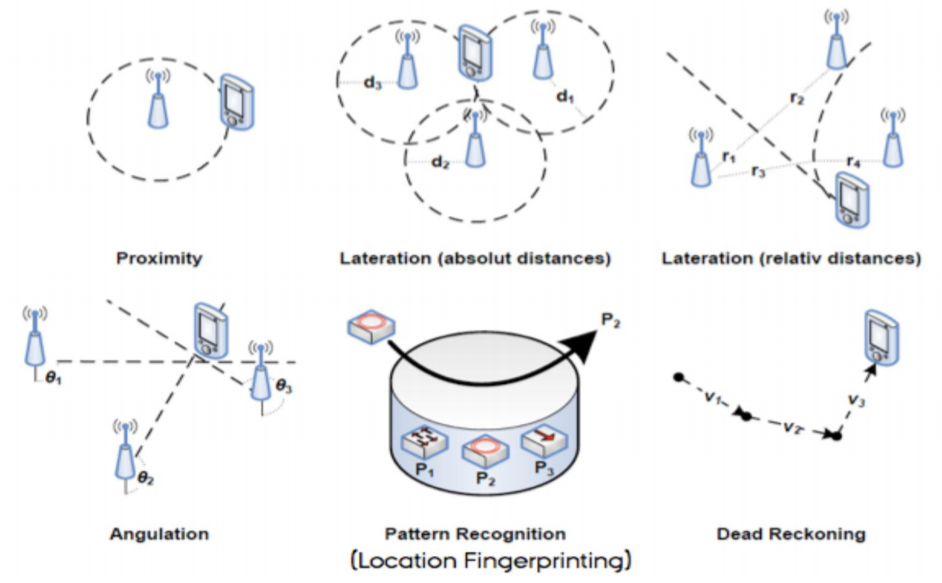
\includegraphics[scale=0.35]{fig5-lec3pt1.png}
    \caption{Tecniche di Geolocalizzazione}
    \label{fig:fig5-lec3pt1}
\end{figure}

\subsection{Tecniche Geometriche}\label{subsubsec3.5.1}

Tra le tecniche di geolocalizzazione geometriche abbiamo:
\begin{itemize}
    \item Laterazione/Trilaterazione: usa l'informazione sulla
    distanza dal nodo anchor per localizzare il nodo. In assenza di rumore e se si
    assume che il segnale radio assuma la forma circolare è sufficiente risolvere un
    sistema di equazioni lineari e la posizione è l'intersezione tra i cerchi. Se
    invece c'è rumore, la posizione è l'area.
    \item Bounding-Box (Min-Max): metodo più efficiente della
    trilaterazione dal punto di vista computazionale, ma meno accurato. Si
    costruiscono dei rettangoli intorno ai nodi anchor e la posizione del nodo
    sconosciuto si trova nel rettangolo di intersezione: da notare che il
    rettangolo è quello in cui è inscritto il cerchio di prima. Anche in questo caso
    la posizione si trova risolvendo delle equazioni lineari.
    \item Triangolazione: per calcolare la posizione si sfruttano le
    proprietà dei triangoli. Tutte le misurazioni fatte si basano sulle tecniche AoA
    (Angle of Arrival).
    \item Multilaterazione: sfrutta la misura TDoA (Time Difference
    of Arrival) per cui il segnali di un nodo sconosciuto è misurato da diversi nodi
    anchor.
    \item Closest-Neighbor: localizzazione basata sulla prossimità.
\end{itemize}
% \end{document}
